\documentclass[letterpaper,10pt]{article}
\usepackage[margin=0.3in]{geometry}
\usepackage{multicol}
\usepackage{amsmath,amssymb}
\usepackage{enumitem}
\usepackage{titlesec}
\usepackage{fancyhdr}
\usepackage{graphicx}

% Set font to sans-serif for clarity
\renewcommand{\familydefault}{\sfdefault}
\usepackage{helvet}

% Set section fonts to 7pt
\usepackage{anyfontsize}
\usepackage{sectsty}
\sectionfont{\fontsize{7}{8}\selectfont}
\subsectionfont{\fontsize{7}{8}\selectfont}
\subsubsectionfont{\fontsize{7}{8}\selectfont}

% Remove page numbers
\pagestyle{fancy}
\fancyhf{}
\renewcommand{\headrulewidth}{0pt}
\renewcommand{\footrulewidth}{0pt}

% Adjust spacing before and after section titles
\usepackage{titlesec}
\titlespacing*{\section}{0pt}{0pt}{0pt} % 0pt before, 0pt after
\titlespacing*{\subsection}{0pt}{0pt}{0pt} % 0pt before, 0.5pt after
\titlespacing*{\subsubsection}{0pt}{0pt}{0pt} % 0pt before, 0pt after

\let\oldsection\section
\renewcommand{\section}[1]{%
\vspace{-1em}
  \oldsection{#1}% Print the original section
  \par\vspace{-2em}% Adjust vertical spacing as needed
  \noindent\rule{0.5\textwidth}{0.5pt}% The line
  \vspace{0em}% Some space after the line if desired
}


% Begin document
\begin{document}
\small
\begin{multicols}{2}



\section{Exam/HW 1}
Mathematical modeling of LTI system does not vary over time. \textbf{True}\\
Principle of superposition holds for linear system. \textbf{True}\\
Closed loop system does not need sensors. \textbf{False}\\
Complementary solution of spring-damper system is given as an exponential function. \textbf{True}\\
Mass-spring-damper system is a second-order system. \textbf{True}\\
Laplace transformation is a nonlinear operator. \textbf{False}\\
Laplace transform of a unit step function is $1/s$. \textbf{True}\\
Laplace transform of differentiation does not need initial conditions. \textbf{False}\\
Final val theory, $\lim_{t \to \infty} f(t) = \lim_{s \to 0} sF(s)$, is true for any $f(t)$. \textbf{False}\\
Transfer function is the Laplace transform of the output to the Laplace transform of the input. \textbf{True}
\section{Exam 2}
For step input, DC motor can hold the position. \textbf{False}\\
Type 0 system has no pole at $s = 0$. \textbf{True}\\
For Type 1 system, the steady-state error for step input is zero. \textbf{True}\\
For Type 1 system, the steady-state error for ramp input is $\infty$. \textbf{False}\\
If all coefficients of the characteristic equation are positive, then the system is stable. \textbf{False}\\
For $G_{cl}(s) = \frac{G(s)}{1 + G(s)H(s)}$, root locus can be found with the angle condition $\angle G(s)H(s) = \pm\pi 2n$, where $n$ is an integer, and magnitude condition $|G(s)H(s)| = 1$. \textbf{False}\\
In root locus, the locus starts from poles and ends at zeros. \textbf{True}\\
On the real axis, you can use the angle condition to find the behavior of root locus. \textbf{True}\\
PD controller does not have steady-state error. \textbf{False}\\
Derivative controller makes the controller more responsive (faster response). \textbf{True}

\section{Exam 3}
$\tan^{-1}\left(\frac{1}{1}\right) = \tan^{-1}\left(\frac{-1}{-1}\right)$. \textbf{False}\\
If $\angle G(j\omega) > 0$, we say that the response is leading the input. \textbf{True}\\
Consider the compensator $G_c(s) = K\frac{s + a}{s + b}$. If $b > a$, then it is a lead compensator. \textbf{True}\\
For Bode plot, the magnitude is computed using $10 \log |G(j\omega)|$. \textbf{False}\\
The phase contribution of $G(s) = j\omega$ is $+90^\circ$. \textbf{True}\\
For $G(s) = \frac{1}{Ts + 1}$, the difference between the asymptote and the exact curve at the corner frequency is 10 dB. \textbf{False}\\
High pass filter blocks the signal with high frequency. \textbf{False}\\
The bandwidth frequency is the lowest frequency for which the gain has declined 3 dB below the asymptote level $G(0)$. \textbf{True}\\
For Nyquist stability criterion, $Z$ means the number of zeros of $1 + G(s)H(s)$ in the LHP. \textbf{False}\\
For Nyquist stability criterion, $N$ means the number of clockwise encirclements of the $-1 + j0$ point. \textbf{True}

\section{HW2} \vspace{-0em}
Damper element stores the energy. \textbf{False}\\
Underdamped system has damping ratio between 0 and 1. \textbf{True}\\
The stability of a 2nd order system depends on the sign of the real part of the poles of the transfer function. \textbf{True}\\
If the step response is stable, then the ramp response is stable. \textbf{False}\\
Steady-state error is a specific performance indicator. \textbf{False}\\
For second-order system, overshoot always occurs. \textbf{False}\\
Settling time is always greater than or equal to rise time. \textbf{True}\\
Laplace transformation exists for all time functions. \textbf{False}\\
Initial value theorem can be used to find steady-state error. \textbf{False}\\
Impulse response is the system response with respect to the impulse input. \textbf{True}

% Additional Content (Optional)
\section{Laplace}
\[
\mathcal{L}\left\{\frac{d^n f(t)}{dt^n}\right\} = s^n F(s) - s^{n-1}f(0) - s^{n-2}f'(0) - \cdots - f^{(n-1)}(0)
\]

\section{PFE (Fraction Expansion}
% You can add more sections or content here if needed
\textbf{Method 1: Substituting Strategic Values}\newline
Continuing with \( s = s^2(s + n)^2 \):\newline
After multiplying both sides by the denominator, we have:
\begin{equation*}
s = A \cdot s(s + n)^2 + B \cdot (s + n)^2 + C \cdot s^2(s + n) + D \cdot s^2
\end{equation*}
\textbf{Choose \( s = 0 \):}
    \begin{equation*}
    0 = A \cdot 0 \cdot (0 + n)^2 + B \cdot (0 + n)^2 + C \cdot 0^2 \cdot (0 + n) + D \cdot 0^2
    \end{equation*}
    \begin{equation*}
    0 = B \cdot n^2 \implies B = 0
    \end{equation*}
\textbf{Choose \( s = -n \):}
    \begin{equation*}
    -n = A \cdot (-n) \cdot 0^2 + B \cdot 0^2 + C \cdot (-n)^2 \cdot 0 + D \cdot (-n)^2
    \end{equation*}
    \begin{equation*}
    -n = D \cdot n^2 \implies D = -\frac{n}{n^2} = -\frac{1}{n}
    \end{equation*}
\newline
\textbf{Method 2: Comparing Coefficients}
\vspace{-0.5em}
\begin{equation*}
s = A \cdot s(s + n)^2 + B \cdot (s + n)^2 + C \cdot s^2(s + n) + D \cdot s^2
\end{equation*}
\vspace{-2em}
\begin{align*}
A \cdot s(s + n)^2 &= A s^3 + 2A n s^2 + A n^2 s, \\
B \cdot (s + n)^2 &= B s^2 + 2B n s + B n^2, \\
C \cdot s^2(s + n) &= C s^3 + C n s^2, \\
D \cdot s^2 &= D s^2.
\end{align*}
\newline
\textbf{Combine All Expanded Terms:}
\begin{equation*}
s = (A s^3 + C s^3) + (2A n s^2 + B s^2 + C n s^2 + D s^2) + (A n^2 s + 2B n s) + B n^2
\end{equation*}
\begin{equation*}
s = (A + C) s^3 + (2A n + B + C n + D) s^2 + (A n^2 + 2B n) s + B n^2
\end{equation*}
\newline
\textbf{Set Up Equations by Matching Coefficients:}
\begin{align*}
\text{For } s^3 &: \quad 0 = A + C, \\
\text{For } s^2 &: \quad 0 = 2A n + B + C n + D, \\
\text{For } s^1 &: \quad 1 = A n^2 + 2B n, \\
\text{For } s^0 &: \quad 0 = B n^2.
\end{align*}

\section{Exam 1, P5}
\subsection*{(a) Mathematical Model:}
The system consists of a mass \(m\), two springs \(k_1, k_2\), and two dampers \(b_1, b_2\). The total force acting on the mass is:

\[
m\ddot{x} = -k_1x - b_1\dot{x} - k_2x - b_2\dot{x} \xrightarrow{} m\ddot{x} + (b_1 + b_2)\dot{x} + (k_1 + k_2)x = 0.
\]
This represents the equation of motion for the system.

\subsection*{(b) Natural Frequency and Damping Ratio:}

Given: \(m = 1 \, \text{kg}, \, b_1 = 2 \, \text{kg/s}, \, b_2 = 4 \, \text{kg/s}, \, k_1 = 10 \, \text{kg/s}^2, \, k_2 = 15 \, \text{kg/s}^2\),
\newline 
the equation of motion becomes:
\[
\ddot{x} + 6\dot{x} + 25x = 0, \quad \text{where } b_1 + b_2 = 6 \, \text{kg/s}, \, k_1 + k_2 = 25 \, \text{kg/s}^2.
\]
\newline
Taking the Laplace transform (assuming zero initial conditions):
\[
[s^2 + 6s + 25]X(s) = 0.
\]
\newline
From the standard second-order system form \(s^2 + 2\zeta \omega_n s + \omega_n^2 = 0\), we identify:

\[
\omega_n = \sqrt{\frac{k_\text{total}}{m}} = \sqrt{\frac{25}{1}} = 5 \, \text{rad/s}.
\]
\newline The damping ratio is:

\[
\zeta = \frac{b_\text{total}}{2m\omega_n} = \frac{6}{2(1)(5)} = 0.6.
\]

\section{Final \& Initial Value Theorem}
The \textbf{Final Value Theorem} is given by:
\begin{equation*}
    \lim_{t \to \infty} f(t) = \lim_{s \to 0} s F(s),
\end{equation*}
provided the limits exist and all poles of $F(s)$ are in the left half-plane, except possibly at $s = 0$.
\newline
The \textbf{Initial Value Theorem} is given by:
\begin{equation*}
    \lim_{t \to 0^+} f(t) = \lim_{s \to \infty} s F(s),
\end{equation*}
where $F(s)$ is the Laplace Transform of $f(t)$.

\section{HW1, BP; Single Mass, 2 displacement problem}
The equation of motion for the mass \(m\) is:
\[
m \ddot{x}_o + b_1 (\dot{x}_o - \dot{x}_i) + k_1 (x_o - x_i) + b_2 \dot{x}_o + k_2 x_o = 0
\]

\[
m \ddot{x}_o + (b_1 + b_2) \dot{x}_o + (k_1 + k_2) x_o = b_1 \dot{x}_i + k_1 x_i
\]
Assuming zero initial conditions (\(x_o(0^-) = 0\) and \(x_i(0^-) = 0\)):
\[
m s^2 X_o(s) + (b_1 + b_2) s X_o(s) + (k_1 + k_2) X_o(s) = b_1 s X_i(s) + k_1 X_i(s)
\]
Factorize \(X_o(s)\) on the left-hand side:
\[
X_o(s) \left[ m s^2 + (b_1 + b_2) s + (k_1 + k_2) \right] = X_i(s) \left[ b_1 s + k_1 \right]
\]
Solve for the transfer function \(H(s) = \frac{X_o(s)}{X_i(s)}\):
\[
H(s) = \frac{b_1 s + k_1}{m s^2 + (b_1 + b_2) s + (k_1 + k_2)}
\]
\vspace{-1em} \section{Block Diagrams}
For blocks in series, the transfer functions are multiplied:
\[
G_{\text{eq}}(s) = G_1(s) \cdot G_2(s)
\]
For blocks in parallel, the transfer functions are added:
\[
G_{\text{eq}}(s) = G_1(s) + G_2(s)
\]
For a system with forward path gain \( G(s) \) and feedback path gain \( H(s) \):
\[
T(s) = \frac{G(s)}{1 + G(s)H(s)}
\]

\section{Simplification of Feedback Systems}

Simplifying \( \frac{G}{1 + G} \), where \( G = \frac{N}{D} \)
\[
\frac{G}{1 + G} = \frac{N}{N + D}
\]

Simplifying \( \frac{G}{1 + GH} \), where \( G = \frac{N}{D} \) and \( H = \frac{A}{B} \)
\[
\frac{G}{1 + GH} = \frac{BN}{DB + NA}
\]
\vspace{-2.5em}
\section{Root Locus}

\begin{enumerate}[leftmargin=*]
    \item \textbf{Plot Poles and Zeros}: Mark all poles (\( \times \)) and zeros (\( \circ \)) of \( G(s)H(s) \) on the complex plane.
    
    \item \textbf{Determine Real Axis Segments}: Root locus exists on real axis segments with an odd number of poles and zeros to their right.
    
    \item \textbf{Calculate Asymptotes}:
    \begin{itemize}[leftmargin=*]
        \item \textbf{Number}: \( p - z \) (where \( p \) is number of poles and \( z \) is number of zeros).
        \item \textbf{Angles}: \( \theta = \frac{(2q + 1)180^\circ}{p - z} \), \( q = 0,1,\ldots,p-z-1 \).
        \item \textbf{Centroid}: \( \sigma = \frac{\sum \text{Poles} - \sum \text{Zeros}}{p - z} \).
    \end{itemize}
\end{enumerate}

\section{Second-Order Form}
\[
G(s) = \frac{\omega_n^2}{s^2 + 2\zeta\omega_n s + \omega_n^2}
\]
\section{State Space Representation}
The state-space representation can be written in the form:
\[
\dot{z} = A z + B \begin{bmatrix} u \\ \dot{u} \end{bmatrix}.
\]
A general structure for $A$ and $B$ could look like:
\[
z = \begin{bmatrix} x \\ \dot{x} \\ y \\ \dot{y} \end{bmatrix}, \quad
\dot{z} =
\setlength{\arrayrulewidth}{0.6pt}
\renewcommand{\arraystretch}{1.5}
\begin{array}{c|cccc}
    \hline
    \text{A} & x & \dot{x} & y & \dot{y} \\ \hline
    \dot{x}      & * & *       & * & *       \\
    \ddot{x}     & * & *       & * & *       \\
    \dot{y}      & * & *       & * & *       \\
    \ddot{y}     & * & *       & * & *       \\
\end{array} z
\;+\; 
\setlength{\arrayrulewidth}{0.6pt}
\renewcommand{\arraystretch}{1.5}
\begin{array}{c|cc}
    \hline
    \text{B} & u & \dot{u} \\ \hline
    x            & * & *       \\
    \dot{x}      & * & *       \\
    y            & * & *       \\
    \dot{y}      & * & *       \\
\end{array} u.
\]
Here, the elements denoted by $*$ would be filled in based on the system parameters $m_i$, $k_i$, $b_i$ and how the input $u$ \& $\dot{u}$) enters the system.

\section{Routh}
\noindent Characteristic polynomial (from Denominator):
\[
P(s) = a_n s^n + a_{n-1} s^{n-1} + \cdots + a_1 s + a_0.
\]
\[
\text{1st row: } \{a_n, a_{n-2}, a_{n-4}, \dots\}, \quad
\text{2nd row: } \{a_{n-1}, a_{n-3}, a_{n-5}, \dots\}.
\]
Subsequent rows:
\[
R_{ij} = \frac{R_{i-1,j} \times R_{i-2,j+1} - R_{i-1,j+1} \times R_{i-2,j}}{R_{i-1,j}}.
\]

\[
\begin{array}{c|ccccc|c}
\hline
\textbf{Col (\(j\))} & \mathbf{1} & \mathbf{2} & \mathbf{3} & \mathbf{4} & \mathbf{5} & \textit{Row (\(i\))} \\ \hline
s^8 & a_8 & a_6 & a_4 & a_2 & a_0 & \textit{1} \\
s^7 & a_7 & a_5 & a_3 & a_1 & 0   & \textit{2} \\ 
s^6 & R_{31} & R_{32} & R_{33} & R_{34} & R_{35} & \textit{3} \\ 
s^5 & R_{41} & R_{42} & R_{43} & R_{44} & R_{45} & \textit{4} \\ 
s^4 & R_{51} & R_{52} & R_{53} & R_{54} & R_{55} & \textit{5} \\ 
s^3 & R_{61} & R_{62} & R_{63} & R_{64} & R_{65} & \textit{6} \\ 
s^2 & R_{71} & R_{72} & R_{73} & R_{74} & R_{75} & \textit{7} \\ 
s^1 & R_{81} & R_{82} & R_{83} & R_{84} & R_{85} & \textit{8} \\ 
s^0 & R_{91} & 0      & 0      & 0      & 0      & \textit{9} \\ 
\hline
\end{array}
\]
1. If all elements in the first column have the same sign, stable.
\newline
2. Sign changes in the first column = number of RHP roots.
\newline \textbf{SPECIAL CASES}
\newline
1. If the first element of a row is zero, use \(\epsilon > 0\) and let \(\epsilon \to 0\).
\newline
2. A zero row indicates symmetric or repeated roots. Use the auxiliary polynomial from the row above:
\[
A(s) = a_m s^m + a_{m-2} s^{m-2} + \cdots.
\]
\vspace{-2em}
\newline
2a. Differentiate \(A(s)\) to form a new row.
\section{Bode Plot Summary}
\begin{itemize}
    \item \textbf{Zero (e.g., $s+a$):}
    \begin{itemize}
        \item \textit{Gain:} Increases at $+20\,\text{dB/decade}$ from $\omega = a$.
        \item \textit{Phase:} Starts $+90^\circ$ change 1 decade before $\omega = a$.
    \end{itemize}
    \item \textbf{Pole (e.g., $1/(s+a)$):}
    \begin{itemize}
        \item \textit{Gain:} Decreases at $-20\,\text{dB/decade}$ from $\omega = a$.
        \item \textit{Phase:} Starts $-90^\circ$ change 1 decade before $\omega = a$.
    \end{itemize}
\end{itemize}

\section{Margins}

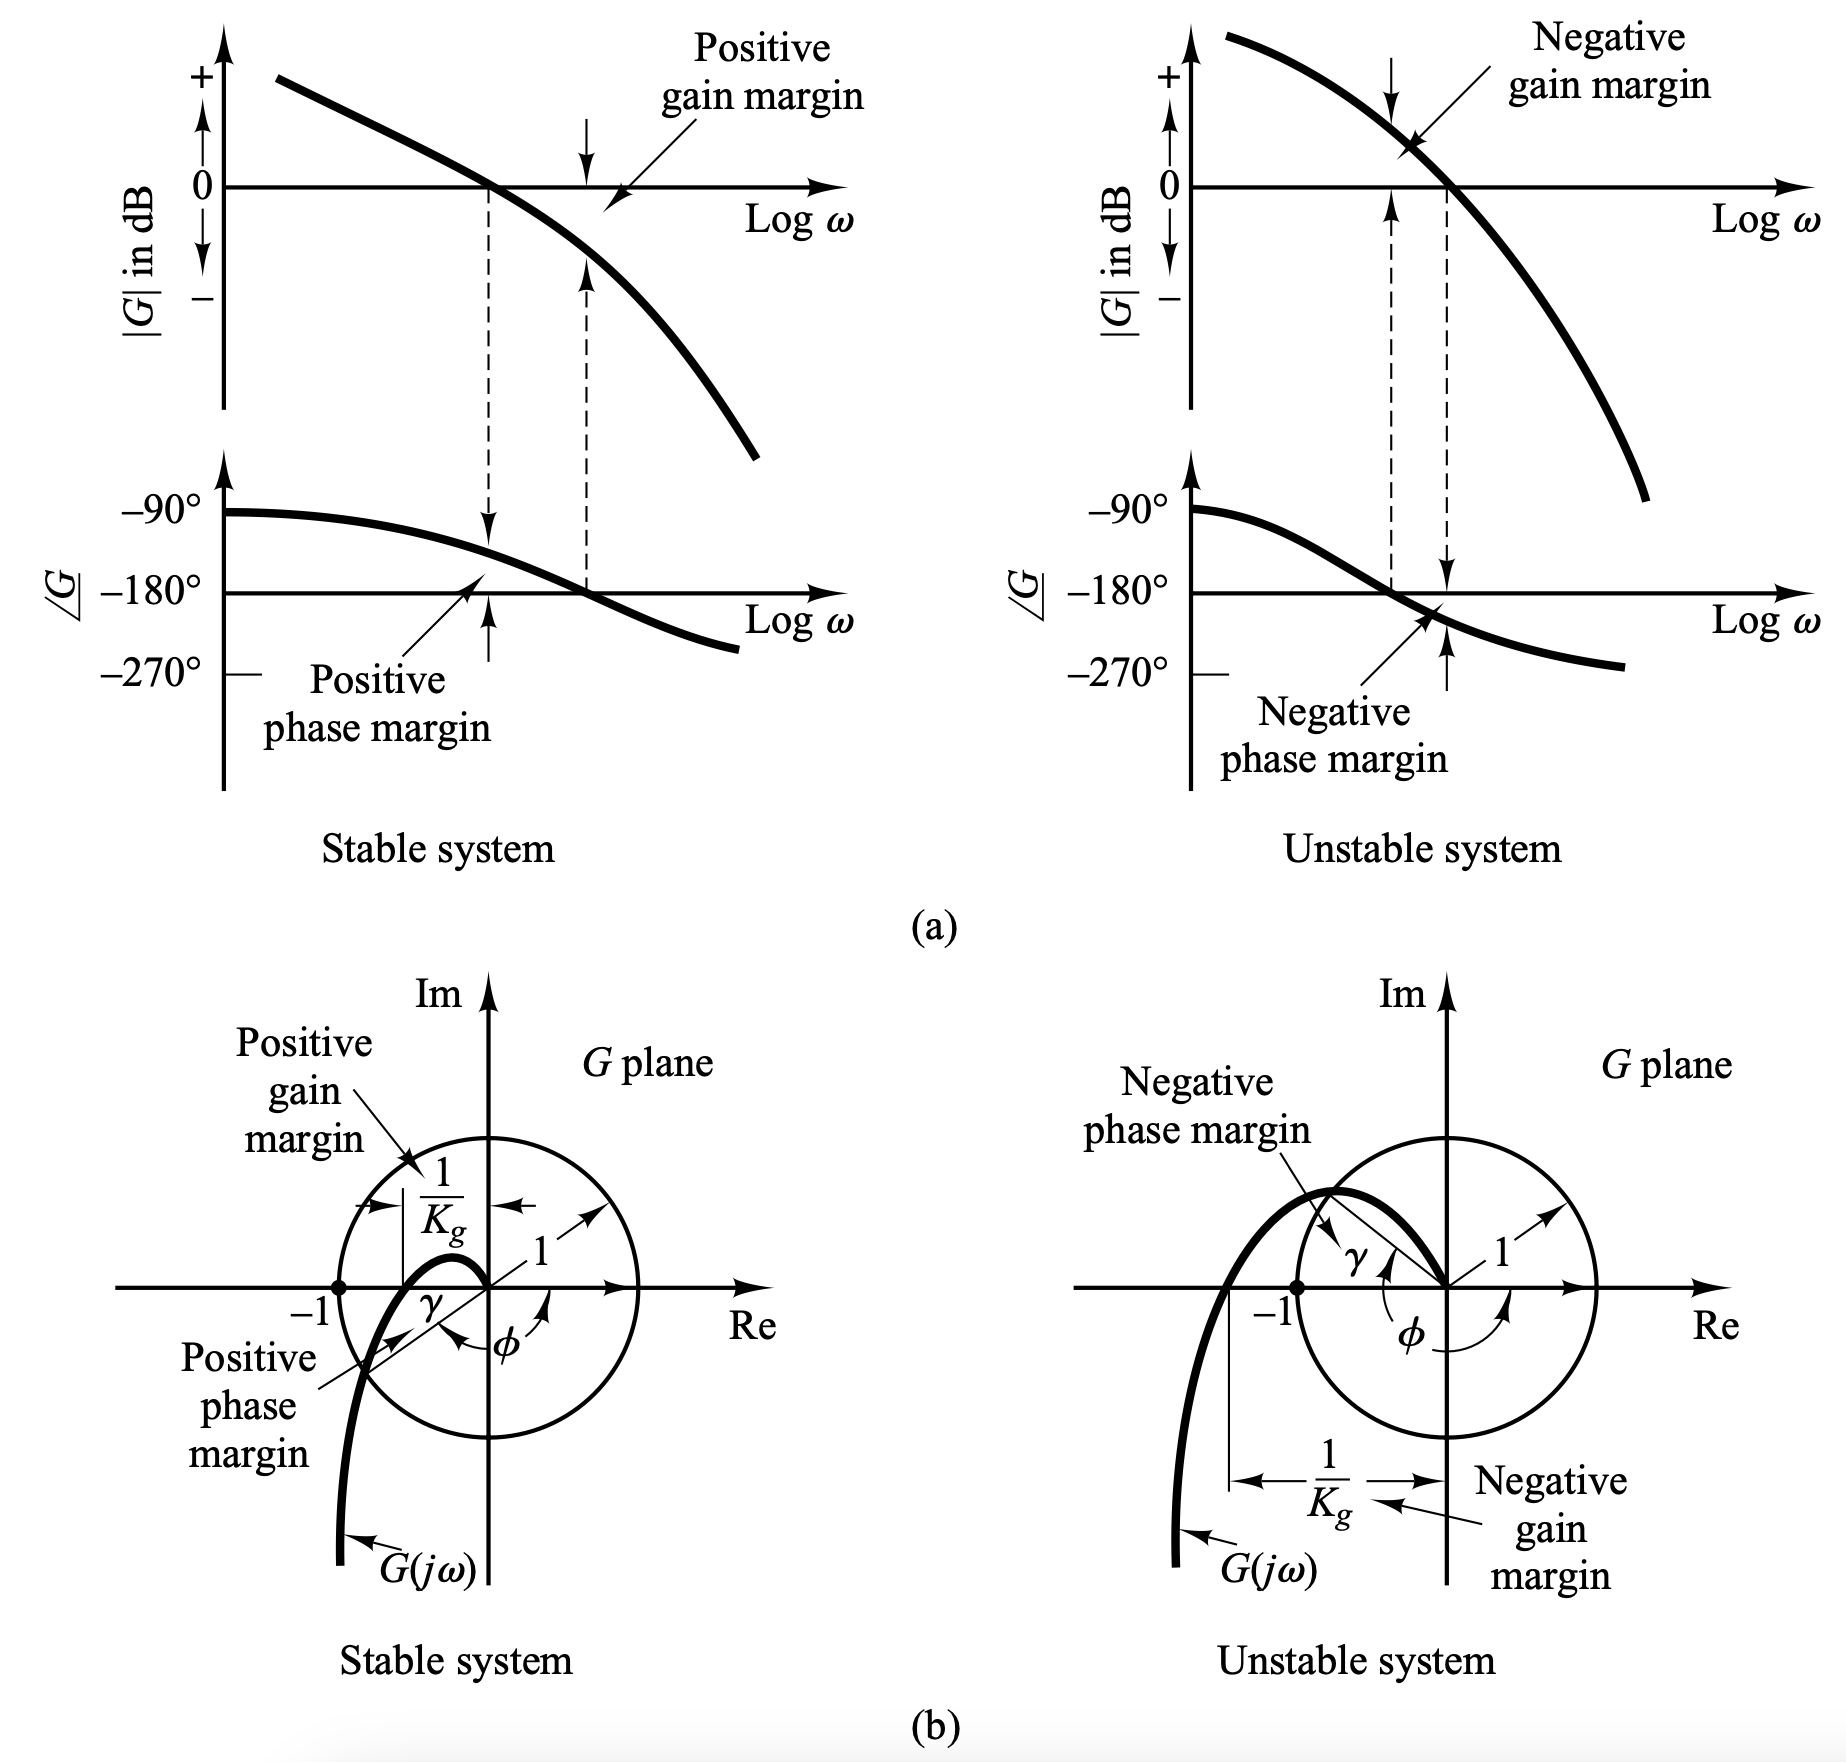
\includegraphics[width=0.95\columnwidth]{Margins.png}

\section{System Type}
\begin{center}
    
\begin{tabular}{|c|c|c|c|}
\hline
\textbf{Type} & \textbf{TF} & \multicolumn{2}{c|}{\textbf{Steady state error}} \\ \cline{3-4} 
              &             & \textbf{Step error} & \textbf{Ramp error} \\ \hline
0             & $\frac{K(T_a s + 1) \cdots}{(T_1 s + 1) \cdots}$ 
              & $\frac{1}{1+K}$ & $\infty$ \\ \hline
1             & $\frac{K(T_a s + 1) \cdots}{s(T_1 s + 1) \cdots}$ 
              & $0$ & $\frac{1}{K}$ \\ \hline
2             & $\frac{K(T_a s + 1) \cdots}{s^2(T_1 s + 1) \cdots}$ 
              & $0$ & $0$ \\ \hline
\end{tabular}
\end{center}

\section{Steady-State Error Analysis}

\subsection*{For Step Input: $U(s) = \frac{1}{s}$}
\[
\lim_{t \to \infty} e(t) = \lim_{s \to 0} \frac{s}{1 + G(s)} U(s) 
= \lim_{s \to 0} \frac{1}{1 + G(s)}
\]

\begin{itemize}
    \item \textbf{Type 0 system:} $\lim_{s \to 0} G(s) = K \implies \lim_{t \to \infty} e(t) = \frac{1}{1+K}$
    \begin{itemize}
        \item Example: DC motor
    \end{itemize}
    \item \textbf{Type 1 system:} $\lim_{s \to 0} G(s) = \infty \implies \lim_{t \to \infty} e(t) = 0$
    \item \textbf{Type 2 system:} $\lim_{s \to 0} G(s) = \infty \implies \lim_{t \to \infty} e(t) = 0$
\end{itemize}

\subsection*{For ramp input: $U(s) = \frac{1}{s^2}$}
\[
\lim_{t \to \infty} e(t) = \lim_{s \to 0} \frac{s}{1 + G(s)} U(s) 
= \lim_{s \to 0} \frac{1}{s + sG(s)}
\]

\begin{itemize}
    \item \textbf{Type 0 system:} $\lim_{s \to 0} sG(s) = 0 \implies \lim_{t \to \infty} e(t) = \infty$
    \item \textbf{Type 1 system:} $\lim_{s \to 0} sG(s) = K \implies \lim_{t \to \infty} e(t) = \frac{1}{K}$
    \item \textbf{Type 2 system:} $\lim_{s \to 0} sG(s) = \infty \implies \lim_{t \to \infty} e(t) = 0$
\end{itemize}
\section{Frequency Analysis}
Given $ G(j\omega)$, and an input $\sin(\omega t +\theta)$, the output is given by

\[
y(t) = X|G(j\omega)| \sin(\omega t + \theta + \phi)
\]

\[
\phi = \angle G(j\omega) = \tan^{-1} \left(\frac{\operatorname{Im}(G(j\omega))}{\operatorname{Re}(G(j\omega))}\right)
\]

\section{Nyquist Stability}

\begin{itemize}
    \item \textbf{Nyquist path:}
    \begin{itemize}
        \item The contour consists of the entire $j\omega$ axis from $\omega = -\infty$ to $\omega = \infty$ and a semicircular path of infinite radius in the RHP.
        \item It encloses the entire RHP $\Rightarrow$ all zeros and poles of $1 + G(s)H(s)$ in RHP.
        \item If there are no zeros of $1 + G(s)H(s)$ in RHP, then there are no closed-loop poles in RHP, and the system is stable.
        \item Nyquist path should not pass through poles or zeros.
    \end{itemize}
    \item \textbf{Mapping theorem:}
    \[
    F(s) = 1 + G(s)H(s)
    \]
    \begin{itemize}
        \item The poles of $F(s)$ = The poles of $G(s)H(s)$.
        \item For closed-loop transfer function, the zeros of $1 + G(s)H(s)$ determine stability.
        \item The number of zeros of $F(s) = 1 + G(s)H(s)$ in the RHP: $Z$.
        \item Relation:
        \[
        N = Z - P \Rightarrow Z = N + P
        \]
        \end{itemize}
    \item \textbf{Summary:} 
        \begin{itemize}
            \item \( Z \): Number of zeros of \( F(s) = 1 + G(s)H(s) \) in the RHP (closed-loop poles).
            \item \( P \): Number of poles of \( G(s)H(s) \) in the RHP (open-loop unstable poles).
            \item \( N \): Net number of encirclements of the critical point \( -1 + 0j \) by the Nyquist plot.
            \item Stability is determined by the equation \( Z = N + P \). If \( Z = 0 \), the system is stable.
        \end{itemize}
    
\end{itemize}

\section{Identifying \( |G(j\omega)| \) and \( \angle G(j\omega) \)}

\subsection*{\( |G(j\omega)| \) (Magnitude):}
\begin{itemize}
    \item \( |G(j\omega)| \) is the magnitude of the transfer function \( G(j\omega) \) at a specific frequency \( \omega \).
    \item To calculate:
    \[
    |G(j\omega)| = \sqrt{\left(\operatorname{Re}(G(j\omega))\right)^2 + \left(\operatorname{Im}(G(j\omega))\right)^2}
    \]
    where:
    \begin{itemize}
        \item \( \operatorname{Re}(G(j\omega)) \): The real part of \( G(j\omega) \).
        \item \( \operatorname{Im}(G(j\omega)) \): The imaginary part of \( G(j\omega) \).
    \end{itemize}
\end{itemize}

\subsection*{\( \angle G(j\omega) \) (Phase):}
\begin{itemize}
    \item \( \angle G(j\omega) \) is the phase angle (argument) of \( G(j\omega) \), describing its rotation in the complex plane.
    \item To calculate:
    \[
    \angle G(j\omega) = \tan^{-1} \left( \frac{\operatorname{Im}(G(j\omega))}{\operatorname{Re}(G(j\omega))} \right)
    \]
    \item Adjust for the correct quadrant as \( \tan^{-1} \) only determines angles in \( [-\pi/2, \pi/2] \).
\end{itemize}

\begin{enumerate}
    \item Segment 1: \((0, j\epsilon) \to (0, jR)\)
    \item Segment 2: \((0, jR) \to (R, 0) \to (0, -jR)\)
    \item Segment 3: \((0, -jR) \to (0, -j\epsilon)\)
    \item Segment 4 (Small semicircle): \(s = \epsilon e^{j\phi}, \phi: -90^\circ \to 0^\circ \to 90^\circ\)
\end{enumerate}

\end{multicols}
\end{document}
